\fancyfoot[C]{Sandri}
\section{Elektrische Antriebsmaschinen}
Elektrische Maschinen wandeln elektrische Energie in mechanische Energie um, indem sie das Prinzip der Lorenzkraft beziehungsweise Reluktanzkraft anwenden um einen Rotor zu rotieren,

\subsubsection{Lorentzkraft}
	Die Lorentzkraft wirkt auf bewegliche Lasungstr�ger in einem Magnetfeld. Sie wirkt senkrecht zur Bewegungsrichtung der Ladung und senkrecht zu den Feldlinien des Magnetfelds. Wie sich die Lorentzkraft verh�lt, l�sst sich anhand folgendem Beispiel, einer Leiterschaukel erkl�ren:\cite{schullv.de2024}

	\begin{figure}[H]
			\centering
			\includegraphics[scale=0.8]{./3_Stand_der_Technik/Abbildungen/Leiterschaukel_1}
			\caption{�nderung der Stromrichtung Lorentzkraft\cite{schullv.de2024}}
	\end{figure}
	
	Die Richtung in welche die Leiterschaukel ausschl�gt, ist zum einen Abh�ngig von der Richtung des Stroms und zum anderen von der Orientierung des Magnetfelds.
	
	\begin{figure}[H]
			\centering
			\includegraphics[scale=0.8]{./3_Stand_der_Technik/Abbildungen/Leiterschaukel_2}
			\caption{�nderung des Magnetfelds Lorentzkraft\cite{schullv.de2024}}
	\end{figure}
	
	Die Richtung der Lorentzkraft kann auch durch einen einfachen Versuch, den linke Hand Versuch, ermittelt werden:
	
	\begin{figure}[H]
			\centering
			\includegraphics[scale=0.8]{./3_Stand_der_Technik/Abbildungen/Lorentzkraft_1}
			\caption{Die linke Hand Regel\cite{schullv.de2024}}
	\end{figure}

	Mathematisch kann die Richtung der Lorentzkraft mihilfe des Kreuzprodukts aus der Magnetfeldrichtung und der Bewegungsrichtung der Elektronen errechnet werden:
	
	\begin{equation}
		\vec{F_{L}} = q * (\vec{v_{e}} \times \vec{B})
	\end{equation}
	
	Der Betrag kann wiefolgt errechnet werden:
	
	\begin{equation}
		F_{L} = q*v*B*\sin{\alpha}
	\end{equation}
	
	Wobei der Winkel $\alpha$ den Winkel zwischen der Bewegungsrichtung der Elektronen und der Bewegungsrichtung des Magnetfelds entspricht. 

\subsubsection{Reluktanzkraft}
	
	\subsection{Asynchronmaschine}
	Die Asynchronmaschine ist die einfachste Form einer elektrischen Maschine. Sie wird angetrieben durch ein Drehfeld, welches durch eine mehrstr�ngige Wicklung im Stator erzeugt wird. Der gro�e Vorteil des Asynchronmaschine ist ihre einfache Bauform und Funktionsweise. Auch bedarf sie nur geringer Wartung. Der gro�e Nachteil hingegen ist jedoch seine startk an die Frequenz der Eingangsspannung gebundene Drehzahl. Im gebr�uchlichen 50-Hz-Betrieb sind nur Drehzahlen von 3000U/min, 1500U/min, 1000U/min, abh�ngig von der Anzahl der Polpaare.
	
	\begin{equation}
		n \thickapprox f / p
	\end{equation}
	
	n $\cdots$ Motordrehzahl \newline
	f $\cdots$ Frequenz vom Netz	\newline
	p $\cdots$ Anzahl der Polpaare \newline
	
	Es gibt haupts�chlich zwei Typen der Asynchronmaschine, den K�figl�ufer und den Schleifringl�ufer. Der K�figl�ufer verwendet also Rotor eines Stahlk�fig, der Schleifringl�ufer hat Schleifringe, �ber die Wicklungen im Rotor bestromt werden.
	
	\begin{figure}[H]
			\centering
			\includegraphics[scale=0.6]{./3_Stand_der_Technik/Abbildungen/Asynchronmaschine_2}
			\caption{Aufbau K�figl�ufer\cite{kfzaufgaben.de2024}}
	\end{figure}
	
	\begin{figure}[H]
			\centering
			\includegraphics[scale=2]{./3_Stand_der_Technik/Abbildungen/Asynchronmaschine_3}
			\caption{Aufbau Schleifringl�ufer\cite{wupperindustrie.de2024}}
	\end{figure}

	Betrieben wird die Asynchronmaschine indem sie an das 3-phasige 50Hz-Netz angeschlossen wird. Sie dreht sich dadurch fast synchron mit der Netzfrequenz. Asynchronmaschinen laufen ihrem Feld jedoch immer etwas hinterher, diese Eigenschaft nennt man Schlupf. Das Drehmoment- und Drehzahlverhalten kann sehr gut mittels eines Kreisdiagramms dargestellt werden.\cite{Fischer2017}
	
	\begin{figure}[H]
			\centering
			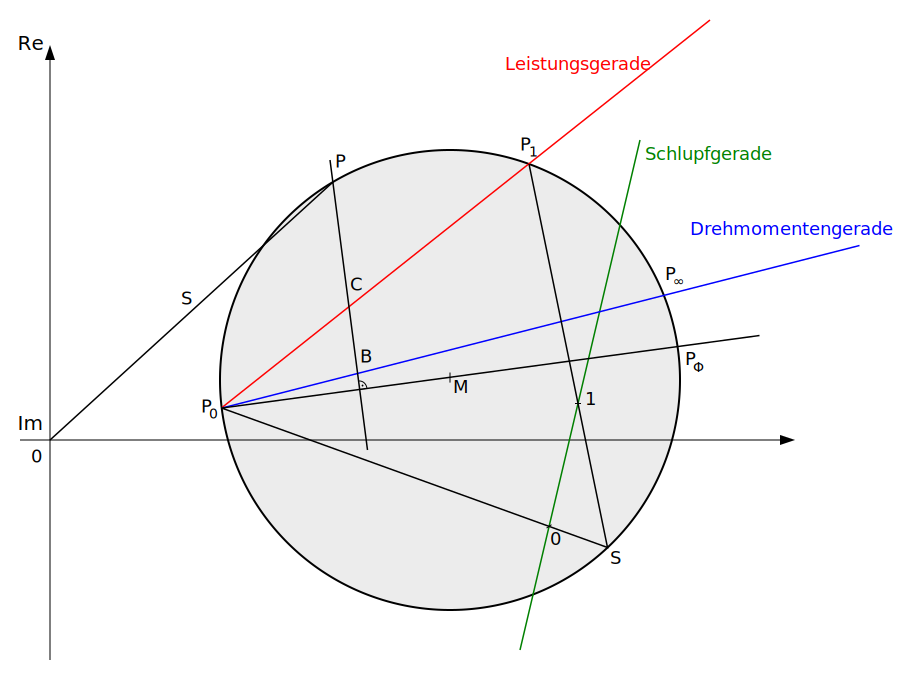
\includegraphics[scale=0.4]{./3_Stand_der_Technik/Abbildungen/Kreisdiagramm_1}
			\caption{Kreisdiagram einer Asynchronmaschine\cite{Wikipedia2024}}
	\end{figure}
	
	
	
	\subsection{Gleichstrommaschine}
	Die Gleichstrommascheine besteht im Stator entweder aus Permanetmagneten, oder aus permanent-erregten Erregerwicklung. Der Rotor besteht aus Wicklungen, welche durch einen Kommutator (auch Stromwender genannt) und B�rsten mithilfe von Gleichspannung versorgt werden. Die Drehzahl der Maschine kann hierbei ganz einfach durch Ver�ndern der Versorgungsspannung linear geregelt werden. 
	
	\begin{figure}[H]
			\centering
			\includegraphics[scale=0.8]{./3_Stand_der_Technik/Abbildungen/Gleichstrommaschine_1}
			\caption{Aufbau Gleichstrommaschine\cite{Pischtschan2024}}
	\end{figure}
	
	Vorteil des Gleichstrommotors ist seine einfach Drehzahlregelung durch Ver�nderung der Spannung, Nachteil der hohe Wartungsaufwand und Verschlei� der Maschine. Er wird aufgrund von sinkenden Preisen bei Frequenzumrichtern immer weniger verwendet.
	
	\input{./3_Stand_der_Technik/7.3_FE_Synchronmaschine}
	
	\input{./3_Stand_der_Technik/7.4_PE_Synchronmaschine}
	
	\input{./3_Stand_der_Technik/7.5_Positionsmessung}
	
	\subsection{Trapezf�rmige Regelung}
%%BLDC Motor wird auch Blockstrommotor genannt
%%evtl noch Schrittmotor inkludieren
	
	\input{./3_Stand_der_Technik/7.7_FOC_Regelung}